\documentclass[12pt,a4paper,final,oneside]{report}
\usepackage{graphics}
\usepackage{graphicx}
\usepackage{listings}
\usepackage{longtable}
\usepackage{underscore}
\usepackage[bookmarks=true]{hyperref}
\hypersetup{
    bookmarks=false,
    pdftitle={Software Project Management Plan},
    pdfauthor={Yiannis Lazarides},
    pdfsubject={TeX and LaTeX},
    pdfkeywords={TeX, LaTeX, graphics, images}, 
    colorlinks=true,       
    linkcolor=blue,       
    citecolor=black,       
    filecolor=black,        
    urlcolor=purple,        
    linktoc=page
}
\def\myversion{1.0 }
\title{%
\flushright
\rule{16cm}{5pt}\vskip1cm
\Huge{Software Project Management Plan}\\
\vspace{0.1cm}
for\\
\vspace{0.1cm}
Speech to 3D Scene Generation\\
\vspace{1cm}
Prepared by\linebreak Manthan Turakhia - 1624013\linebreak Umang Nandu - 1624016 \linebreak Prayesh Shah - 1624019 \linebreak Siddharth Sharma - 1624020\\
\vspace{0.5cm}
Under the guidance of \linebreak Prof. Sagar D. Korde.\\
\vfill
\rule{16cm}{5pt}
}
\date{}
\usepackage{hyperref}
\begin{document}
\maketitle
\tableofcontents
\chapter{Introduction}
\section{Product overview}
\paragraph{}The purpose of the software is to provide a better way for personnel form various industries like creative, corporate and education to present or impart knowledge in a better, more representative, and a more attractive way. As mentioned, the software is targeted for all kinds of professionals and students who are willing to make any kind of a presentation. The expected date for delivery is by 16th March, 2019

\section{Project Deliverables}
\begin{table}[h!]
  \centering

  \begin{tabular}{ |p{2.3cm}| p{6cm} | p{3cm} | }
\hline
    Delivery ID. & Deliverables/work products.& Delivery Date\\
    \hline
    D1. & SRS document which specifies the requirements for project.& 30th Sept..\\
 \hline
    D2. & SPMP Document specifying over all planning and specifying the estimation.& 30th Sept.\\
 \hline
  D2. & SDD Document specifying the designing of system.& 5th Oct.\\
 \hline
  D2. & STD Document specifying the test cases and related information.& 14th Oct.\\
 \hline
    D3. & UML diagrams.& 31st Oct.\\
 \hline
    D4. & UI.& 10th Nov.\\
 \hline
    D5. & Modules.& 10th Jan.\\
 \hline
    D6. &Functional Prototype.& 20th feb.\\
 \hline
   D7. &Application.& 16th March.\\
 \hline
   D8. &Test Report.& 25th March.\\
 \hline

  \end{tabular}
\end{table}
\rule{16cm}{5pt}
\chapter{PROJECT ORGANIZATION}

\section{ Software Process Model}
{Prototyping model}

\paragraph{}The chosen process model is Prototyping model. The Prototyping Model is a systems development method (SDM) in which a prototype (an early approximation of a final system or product) is built, tested, and then reworked as necessary until an acceptable prototype is finally achieved from which the complete system or product can now be developed. This type of working is essential in our project because all the functional requirements need to be tested as a priority. Another important reason behind choosing this model is to make sure that at the end of the day the users get what they want. The software will be modified and updated until the end-game is achieved and the user is completely satisfied.

\section{ Roles and Responsibilities}
\begin{center}
    \begin{tabular}{ |c|c| }
    \hline
    Roles & Responsibilities \\ 
    \hline
    Team Leader& Manage all the tasks and schedules the deadline \\ 
     \hline
  Project Manager & Requirement gathering and coordination of various events.\\ 
    \hline
    Front-end Developer& Development of user friendly user interface.  \\ 
    \hline
   Back-end Developer& Development and linking of various backend modules.\\ 
   \hline
    Tester & Tests all the modules using software testing tools and techniques.\\
\hline
       
    \end{tabular}
\end{center}

\section{ Tools and Techniques}

\begin{enumerate}
\item Texworks to prepare project related documents.
\item IBM Rational Rose for Designing UML Diagrams
]\item PyCharm for python programming.
\end{enumerate}
\rule{16cm}{5pt}
\chapter{Project Management  Plan}
\section{Tasks}\begin{tabular}{ |p{3.5cm}| p{3.5cm} | p{3.5cm} | p{3.5cm}| }
\hline
Tasks& Deliverables and Milestones & Resources needed & Dependencies and constraints \\ 
\hline
Gather Requirements . &SRS document which specifies the requirements for project.& Latex Editor&User’s Approval \\ 
\hline
Confirmation of idea  & SRS document specifies the functional and non-functional requirements. &Latex Editor&Stakeholders approval.\\
 \hline
Planning& SPMP Document specifying over all planning and specifying the estimation.&Latex Editor.&Stakeholders and users involvement.\\ 
\hline
Content Audit.&&Content Analysis Tool.& Evaluating content elements and information assets\\ 
\hline
Visual Design.&UI.&&\\
 \hline
Model Designing.&UML diagrams&IBM Rational Rose.&Approval from RTO.\\ 
\hline
Prototype Development.&Functional Prototype && Creating a basic functional prototype\\ 
\hline
Programming and Re-Engineering.& Modules.& Python IDE, Libraries, packages.& Gather end user feedback and alter if needed. \\ 
\hline
Linking.&Application.&Python IDE.& \\
 \hline
Testing .&Test Report.&Unit Testing tools.&Constructed classes and various modules of the project.\\ 
\hline
Modification .&&&Approval of tester and end user.\\ 
\hline
\end{tabular}

\begin{table}[]\section{Risk Table}
\centering

\label{Risk Table}
\begin{tabular}{|p{3.5cm}| p{2cm} | p{2.3cm} | p{4cm}|}
\hline
Risks                                         & Category  & Impact &Contingencies \\ \hline
Late Delivery                                & BU               & 2   &  Justification. \\ \hline
Computer Crash                                 & TI              & 1 & Accessing backups.   \\ \hline
Technology will not Meet Expectations         & TE            & 1    & Taking feedback and modification. \\ \hline
Deviation from Software Engineering Standards       & PI               & 3  & Slight modifications if necessary.  \\ \hline
Lack of Database Stability                & TI             & 2   &  Making sure of a reliable database like Google 3D Warehouse. \\ \hline
Poor Comments in Code                         & TI              & 4  & Separate manual for developers.   \\ \hline
User’s Disapproval                            & CRR             & 1   & Using prototyping model.  \\ \hline
Changes in Requirements                                & PS             & 2   &  Using prototyping model. \\ \hline
No internet connection                        & TI             & 2  &    \\ \hline
\end{tabular}
\end{table}

\section{ Timetable}

\begin{figure}[h] 
\begin{center} 
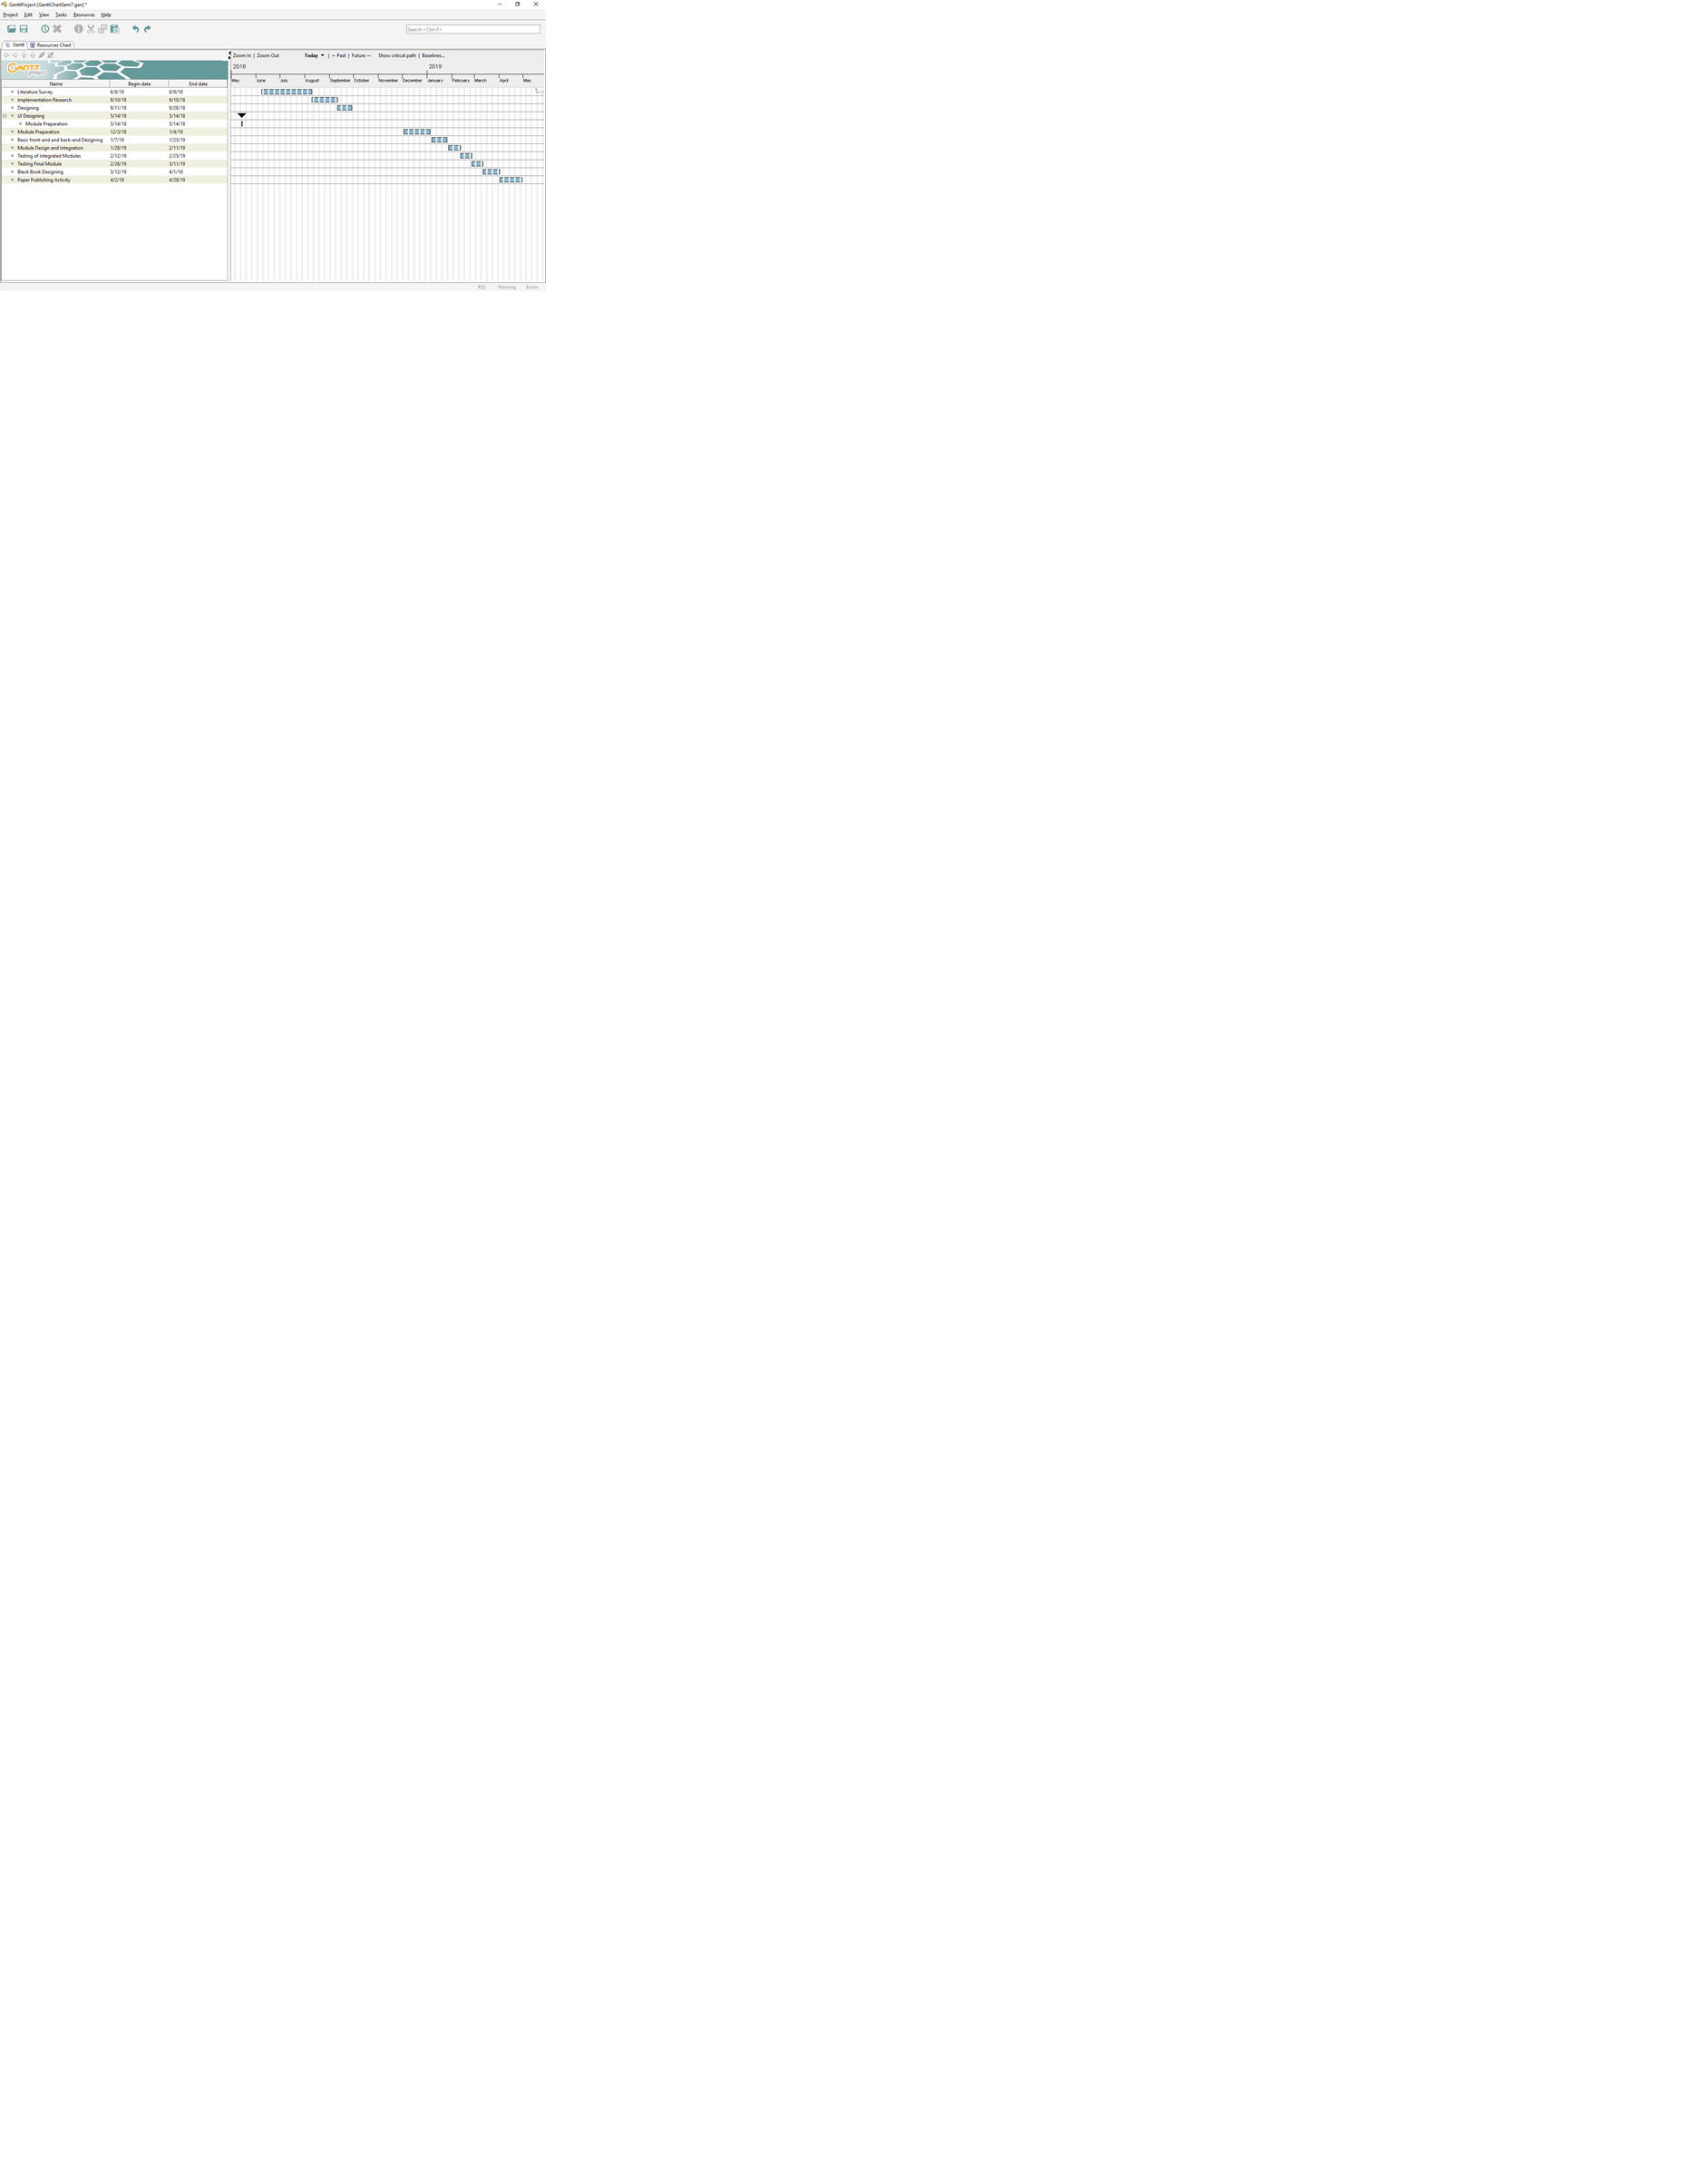
\includegraphics[width=1300px]{gantt.png} \caption{Gantt} 
\end{center}
\end{figure}

\end{document}